% ============================================================
% Lecture 15 -- Estimating the coefficients of linear models
% ============================================================
\section{Estimating the Coefficients of Linear Models}\label{sec:L15}

\lectureheader{15}{qF9VBw3CP78}{Week-5 R code \texttt{Feb21.r} (least squares fit of \texttt{iris}, normal equations by hand) and Week-5 assignment Q4. The Week-5 lecture PDF was \emph{not} accessed. The derivations below follow the titles and code and are marked accordingly.}

\begin{guiding*}
By the end of this lecture you should be able to:
\begin{itemize}
  \item compute $\hat\beta=(X\T X)^{-1}X\T Y$ for a full-rank model, by hand and in code;
  \item prove that $\hat\beta$ is unbiased with $\Cov(\hat\beta)=\sigma^2(X\T X)^{-1}$;
  \item derive $\Var(\hat\beta_0)$, $\Var(\hat\beta_1)$ and $\Cov(\hat\beta_0,\hat\beta_1)$ in simple linear regression;
  \item fit and plot a regression line with \texttt{lm}/\texttt{statsmodels}.
\end{itemize}
\end{guiding*}

\subsection{Recap}
Week~4 established that least squares estimates are the solutions of the normal equations
$X\T X\beta=X\T Y$ (\cref{thm:L12-normal}). The solution is unique iff $\rank X=p$
(\cref{cor:L12-fitted}), and $X\hat\beta=\PX Y$ (\cref{prop:L14-PX}). Week~5 applies this theory to
regression models, which in practice almost always have a full-rank $X$. Throughout this chapter we
write simple linear regression as
\[
Y_i=\beta_0+\beta_1x_i+\eps_i,\qquad i=1,\dots,n,
\]
the notation of the R output (``\texttt{(Intercept)}'' and the slope). In Week~2 we called these
coefficients $a_1,a_2$.

\subsection{The iris example from the R code}
\begin{example}[Sepal length on petal width]\label{ex:L15-iris}
The R code fits \texttt{lm(Sepal.Length \textasciitilde\ Petal.Width, data = iris)} to Fisher's iris data
($n=150$ flowers), plots the points, and adds the fitted line with \texttt{abline} and with
\texttt{ggplot(...) + stat\_smooth(method = "lm")}. The estimates are
\[
\hat\beta_0=4.7776,\qquad \hat\beta_1=0.8886 .
\]
A flower whose petals are $1$\,cm wider has, on average, sepals $0.89$\,cm longer. The line
passes through $(\bar x,\bar y)=(1.1993,\,5.8433)$ (\cref{cor:L05-props}).
\end{example}

\begin{figure}[ht]
\centering
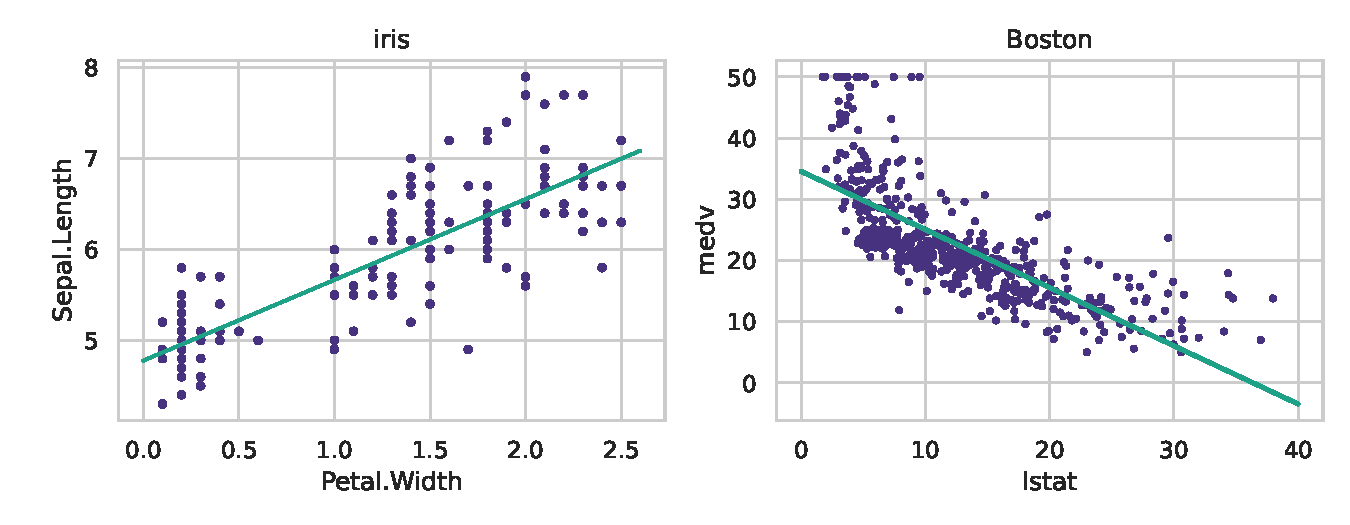
\includegraphics[width=0.95\textwidth]{figures/L15_iris_boston.pdf}
\caption{Least squares lines for \texttt{iris} (\cref{ex:L15-iris}) and for \texttt{Boston} (\cref{sec:L16}).}
\label{fig:L15-fits}
\end{figure}

\subsection{Normal equations by hand}
The second part of the R code solves the normal equations directly for a model with two
explanatory variables:
\begin{center}
\begin{minipage}{0.85\textwidth}\small\ttfamily
x1 <- c(10,0,45,56,79); x2 <- c(2,34,15,5,4)\\
y <- x1 + x2 + rnorm(5, mean=0, sd=0.3)\\
X <- as.matrix(cbind(1,x1,x2))\\
betahat = solve(t(X) \%*\% X) \%*\% (t(X) \%*\% Y) \quad \# solution of X\textasciicircum TX beta = X\textasciicircum Ty\\
lm.fit <- lm(y \textasciitilde\ 1+x1+x2); lm.fit\$coefficients
\end{minipage}
\end{center}
The data are simulated from $Y_i=0+1\cdot x_{1i}+1\cdot x_{2i}+\eps_i$ with $\sigma=0.3$, so $\hat\beta$ should be
close to $(0,1,1)$. Here $n=5$, $p=3$, and
\[
X\T X=\begin{pmatrix}5&190&60\\190&11502&1291\\60&1291&1426\end{pmatrix}.
\]
Its determinant is non-zero ($\rank X=3$), so \texttt{solve} works. The two computations agree. The
exact numbers depend on the random draw. With the notebook's seed they are
$\hat\beta=(0.3665,\ 0.9905,\ 1.0068)$. Different runs of the R code give different numbers, because the
original code sets no seed.

\subsection[Unbiasedness and covariance of the estimator]{Unbiasedness and covariance of \texorpdfstring{$\protect\hat\beta$}{beta-hat}}
\begin{theorem}\label{thm:L15-moments}
Let $(Y,X\beta,\sigma^2I_n)$ be a linear model with $\rank X=p$, and let $\hat\beta=(X\T X)^{-1}X\T Y$. Then
\[
\EE[\hat\beta]=\beta,\qquad \Cov(\hat\beta)=\sigma^2(X\T X)^{-1}.
\]
\end{theorem}
\begin{proof}
$\hat\beta=AY$ with the fixed matrix $A=(X\T X)^{-1}X\T$. By \cref{prop:L09-rules},
$\EE\hat\beta=A\,X\beta=(X\T X)^{-1}X\T X\beta=\beta$. Also
\[
\Cov(\hat\beta)=A(\sigma^2I)A\T=\sigma^2(X\T X)^{-1}X\T X(X\T X)^{-1}=\sigma^2(X\T X)^{-1},
\]
using the symmetry of $(X\T X)^{-1}$.
\end{proof}

\begin{corollary}[Simple linear regression; Week-5 assignment Q4]\label{cor:L15-slr}
For $Y_i=\beta_0+\beta_1x_i+\eps_i$ with the $x_i$ not all equal,
\[
X\T X=\begin{pmatrix}n&\sum x_i\\\sum x_i&\sum x_i^2\end{pmatrix},\qquad X\T Y=\begin{pmatrix}\sum Y_i\\\sum x_iY_i\end{pmatrix},
\]
$\hat\beta_1=S_{xY}/S_{xx}$, $\hat\beta_0=\bar Y-\hat\beta_1\bar x$, and
\[
\Var(\hat\beta_1)=\frac{\sigma^2}{S_{xx}},\qquad
\Var(\hat\beta_0)=\sigma^2\Bigl(\frac1n+\frac{\bar x^2}{S_{xx}}\Bigr),\qquad
\Cov(\hat\beta_0,\hat\beta_1)=-\frac{\sigma^2\bar x}{S_{xx}} .
\]
\end{corollary}
\begin{proof}
The formulas for $X\T X$, $X\T Y$ and $\hat\beta$ are \cref{prob:L12-1}. Now $\det(X\T X)=n\sum x_i^2-(\sum x_i)^2=nS_{xx}$, so
\[
(X\T X)^{-1}=\frac1{nS_{xx}}\begin{pmatrix}\sum x_i^2&-\sum x_i\\-\sum x_i&n\end{pmatrix}.
\]
By \cref{thm:L15-moments}: $\Var(\hat\beta_1)=\sigma^2 n/(nS_{xx})=\sigma^2/S_{xx}$ and
$\Cov(\hat\beta_0,\hat\beta_1)=-\sigma^2 n\bar x/(nS_{xx})=-\sigma^2\bar x/S_{xx}$. For the intercept,
$\Var(\hat\beta_0)=\sigma^2\sum x_i^2/(nS_{xx})$, and $\sum x_i^2=S_{xx}+n\bar x^2$ gives
$\sigma^2(1/n+\bar x^2/S_{xx})$.

A direct check without matrices: $\hat\beta_1=\sum_i c_iY_i$ with $c_i=(x_i-\bar x)/S_{xx}$, so
$\Var(\hat\beta_1)=\sigma^2\sum c_i^2=\sigma^2S_{xx}/S_{xx}^2$. Also $\Cov(\bar Y,\hat\beta_1)=\frac{\sigma^2}{n}\sum c_i=0$.
Then $\Var(\hat\beta_0)=\Var(\bar Y)+\bar x^2\Var(\hat\beta_1)-2\bar x\Cov(\bar Y,\hat\beta_1)$, which gives the same result.
\end{proof}

\begin{example}[The hand example again]\label{ex:L15-hand}
For $x=(1,2,3,4)$ (\cref{ex:L12-slr}): $n=4$, $\bar x=2.5$, $S_{xx}=5$, and
\[
(X\T X)^{-1}=\frac1{20}\begin{pmatrix}30&-10\\-10&4\end{pmatrix}=\begin{pmatrix}1.5&-0.5\\-0.5&0.2\end{pmatrix}.
\]
So $\Var(\hat\beta_1)=0.2\sigma^2=\sigma^2/5$, $\Var(\hat\beta_0)=1.5\sigma^2=\sigma^2(1/4+6.25/5)$ and
$\Cov(\hat\beta_0,\hat\beta_1)=-0.5\sigma^2=-2.5\sigma^2/5$, in agreement with \cref{cor:L15-slr}. The
correlation of the two estimates is $-0.5/\sqrt{1.5\times0.2}=-0.913$. Because all $x_i>0$, overestimating the
slope goes with underestimating the intercept.
\end{example}

\begin{note}[Supplementary: design matters]
$\Var(\hat\beta_1)=\sigma^2/S_{xx}$ is small when the $x_i$ are spread out. To estimate a slope well, take
observations far apart. $\Var(\hat\beta_0)$ is smallest when $\bar x=0$. Centring the covariate ($x_i-\bar x$)
makes $\hat\beta_0=\bar Y$ and the two estimates uncorrelated.
\end{note}

\subsection{Computation}
\begin{center}\small
\begin{tabular}{@{}>{\raggedright\arraybackslash}p{7cm}>{\raggedright\arraybackslash}p{8.4cm}@{}}\hline
R & Python\\\hline
\texttt{lm(Sepal.Length \textasciitilde\ Petal.Width, iris)} & \texttt{smf.ols("Sepal\_Length \textasciitilde\ Petal\_Width", ir).fit()}\\
\texttt{abline(fit1)} & \texttt{ax.plot(xs, b0 + b1*xs)}\\
\texttt{stat\_smooth(method="lm")} & \texttt{sns.regplot(...)}\\
\texttt{solve(t(X)\%*\%X) \%*\% t(X)\%*\%Y} & \texttt{np.linalg.solve(X.T @ X, X.T @ Y)}\\
\texttt{vcov(fit)} & \texttt{fit.cov\_params()}\\\hline
\end{tabular}
\end{center}
\nb{week05/L15\_estimating\_coefficients.ipynb} also checks $\Cov(\hat\beta)=\sigma^2(X\T X)^{-1}$ by simulation.

\subsection{Summary}
\begin{itemize}
  \item Full rank: $\hat\beta=(X\T X)^{-1}X\T Y$, $\EE\hat\beta=\beta$, $\Cov\hat\beta=\sigma^2(X\T X)^{-1}$.
  \item SLR: $\Var\hat\beta_1=\sigma^2/S_{xx}$, $\Var\hat\beta_0=\sigma^2(1/n+\bar x^2/S_{xx})$, $\Cov=-\sigma^2\bar x/S_{xx}$.
  \item \texttt{iris}: $\widehat{\text{Sepal.Length}}=4.7776+0.8886\,\text{Petal.Width}$.
\end{itemize}

\subsection{Exercises}
\begin{problem}\label{prob:L15-1}
Show that $\hat\beta_1=\sum_ic_iY_i$ with $c_i=(x_i-\bar x)/S_{xx}$, and that $\sum c_i=0$, $\sum c_ix_i=1$.
\end{problem}
\begin{problem}\label{prob:L15-2}
For $x=(-1,0,1)$, compute $\Cov(\hat\beta)$ in simple linear regression. Why are $\hat\beta_0$ and $\hat\beta_1$ uncorrelated here?
\end{problem}
\begin{problem}\label{prob:L15-3}
Show that $\Var(\hat\beta_0+\hat\beta_1x_0)=\sigma^2\bigl(\frac1n+\frac{(x_0-\bar x)^2}{S_{xx}}\bigr)$.
\end{problem}
\begin{problem}\label{prob:L15-4}
You may choose $n=10$ design points $x_i\in[0,1]$. Which choice minimises $\Var(\hat\beta_1)$?
\end{problem}

\subsection{Further reading}
Christensen, \S2.2 and Chapter~6 (simple linear regression); Rao, \S4a.2; James, Witten, Hastie
\& Tibshirani, \emph{An Introduction to Statistical Learning}, \S3.1 (the source of the lab in the R code).
